\chapter{Différentiabilité dans $\mathbb{C}$}
\section{Rappels de calcul différentiel dans $\R^2$}
Les différentes notions présentées ici sont très classiques et probablement
déjà connues du lecteur. Dans toute cette section, $\Omega$ désignera un ouvert non vide de $\R^2$.
\subsection{Définitions}
\begin{fdefn}
Soit $g \colon \Omega \to \R^+$ une application. On dira que $f \colon \Omega \to \R^2$ est négligeable devant $g$ au
voisinage d'un point $x_0 \in \Omega$ si pour tout $\epsilon > 0$, il existe un voisinage $V_\epsilon$ de $x_0$ tel que:
\[
\forall x \in V_\epsilon, \, \|f(x)\| < \epsilon g(x)
\]
\end{fdefn}
\begin{notation}
On notera l'ensemble des applications négligeable devant $g$ au voisinage de $x_0$ par $o_{x_0}(g)$. 
\end{notation}
\begin{rem}
On condense très souvent la notation $o_{x_0}(g)$ en $o(g)$, le point $x_0$ étant sous-entendu.
\end{rem}
\begin{fdefn}\label{def:1.1}
Soit $\Omega \subset \R^2$ un ouvert et soit une application $f \colon \Omega \to \R^2$.
On dira que $f$ est différentiable en $x_0 \in \Omega$ si il existe une application affine $A \colon \R^2 \to \R^2$ telle
que $f-A \in o(\|x-x_0\|)$
\end{fdefn}
On a nécessairement $A(x_0)=f(x_0)$. En effet, par définition de l'ensemble $o(\|x-x_0\|)$, il existe un voisinage $U$ de $x_0$ tel que:
\[
\forall x \in U, \, \|f(x)-A(x)\| \leq \|x-x_0\|
\]
et la propriété s'ensuit en prenant $x=x_0$.
\begin{prop}
L'application $A$ est unique.
\end{prop}
\begin{proof}
Supposons l'existence d'une application affine $B$ vérifiant la même propriété que $A$. On de façon immédiate que $A-B \in o(\|x-x_0\|)$. Comme $A(x_0)=B(x_0)=f(x_0)$, l'application $\Theta \colon x \mapsto (A-B)(x-x_0)$ est linéaire.
Pour tout $\epsilon > 0$, il existe un voisinage $V_\epsilon$ de $x_0$ tel que:
\[
\forall x \in V_\epsilon, \|\Theta(x-x_0)\| \leq \epsilon \|x-x_0\|
\]
prouvant que la norme de l'application linéaire $\Theta$ est inférieure à $\epsilon$. Ceci étant vrai pour tout $\epsilon$, on en déduit que la norme de $\Theta$ est nulle, montrant ainsi que $\Theta=0$.
\end{proof}
L'application affine $A$ admet une écriture $A=f(x_0) + H(x-x_0)$. On peut ainsi reformuler la définition \ref{def:1.1} comme:
\begin{fdefn}\label{def:1.2}
Soit $\Omega \subset \R^2$ un ouvert et soit une application $f \colon \Omega \to \R^2$.
On dira que $f$ est différentiable en $x_0 \in \Omega$ si il existe une application linéaire $H \colon \R^2 \to \R^2$ telle que:
\[
f-f(x_0)-H(x-x_0) \in o(\|x-x_0\|)
\]
On dit que $H$ est l'application linéaire tangente à $f$ au point $x_0$.
\end{fdefn}
On fait le plus souvent l'abus de notation consistant à confondre \textbf{l'ensemble} $ o(\|x-x_0\|)$ avec un de ses éléments, pour écrire la relation entre $f$ et $H$  au voisinage de $x_0$ sous la forme:
\[
f(x) = f(x_0) + H(x-x_0) + o(\|x-x_0\|)
\]
Cette notation est la plus courante, mais se révèle parfois source d'erreurs: il faut toujours garder à l'esprit
que le terme $o(\|x-x_0\|)$ est en fait une \textbf{fonction} négligeable devant $\|x-x_0\|$ au voisinage de $x_0$.
On notera le plus souvent $H$ par $Df(x_0)$ ou $f^\prime(x_0)$.

Lorsqu'une application est différentiable en un point, elle y est bien représentée par une application linéaire et hérite de certaines de ses propriétés, dont la continuité, comme le montre la proposition ci-dessous:
\begin{fprop}\label{prop:1.1}
Soit $f \colon \Omega \to \R^2$ différentiable en $x_0$. $f$ est continue en $x_0$.
\end{fprop}
\begin{proof}
Soit $\epsilon > 0$. Il existe un voisinage $V_\epsilon$ de $x_0$ tel que:
\[
\forall x \in V_\epsilon, \, \left \| f(x) - f(x_0) -H(x-x_0) \right \| \leq \epsilon \|x-x_0\|
\]
Par ailleurs:
\[
\|f(x) -f(x_0)\| \leq \left \| f(x) - f(x_0) -H(x-x_0) \right \| + \left \| H(x-x_0) \right \|
\]
d où, pour $x \in V_\epsilon$:
\[
\|f(x) -f(x_0)\| \leq \left(\epsilon + \|H\| \right)\|x-x_0\|
\]
On en déduit le résultat.
\end{proof}
Lorsqu'une application est différentiable en tout point d'un ouvert $\Omega$, on dit plus simplement qu'elle est différentiable sur $\Omega$. Il est alors d'usage de noter l'application linéaire tangente à $f$ en $x$ par $f^\prime(x)$. L'application $f^\prime \colon x \in \Omega \mapsto f^\prime(x)$ s'appelle \textbf{application dérivée} de $f$.

\begin{fdefn}
Une application $f \colon \Omega \to \R^2$ différentiable sur $\Omega$ et d'application dérivée continue est dite de classe $C^1(\Omega)$.
\end{fdefn}
\subsection{Interprétation géométrique}

Un endomorphisme de $\R^2$ se représente comme une transformation du plan. Étant linéaire, elle agira sur un segment de droite pour donner un autre segment de droite. La figure \ref{fig:trlin} donne un exemple de l'action d'un endomorphisme du plan sur une grille uniforme ; on notera en particulier que la déformation préserve les parties droites.
\begin{figure}[ht]
\centering
\begin{subfigure}[b]{0.45\textwidth}

\includegraphics[width=\textwidth]{images/ima1.png}
\caption{Grille initiale}
\label{fig:uni_mesh}
\end{subfigure}
\begin{subfigure}[b]{0.45\textwidth}
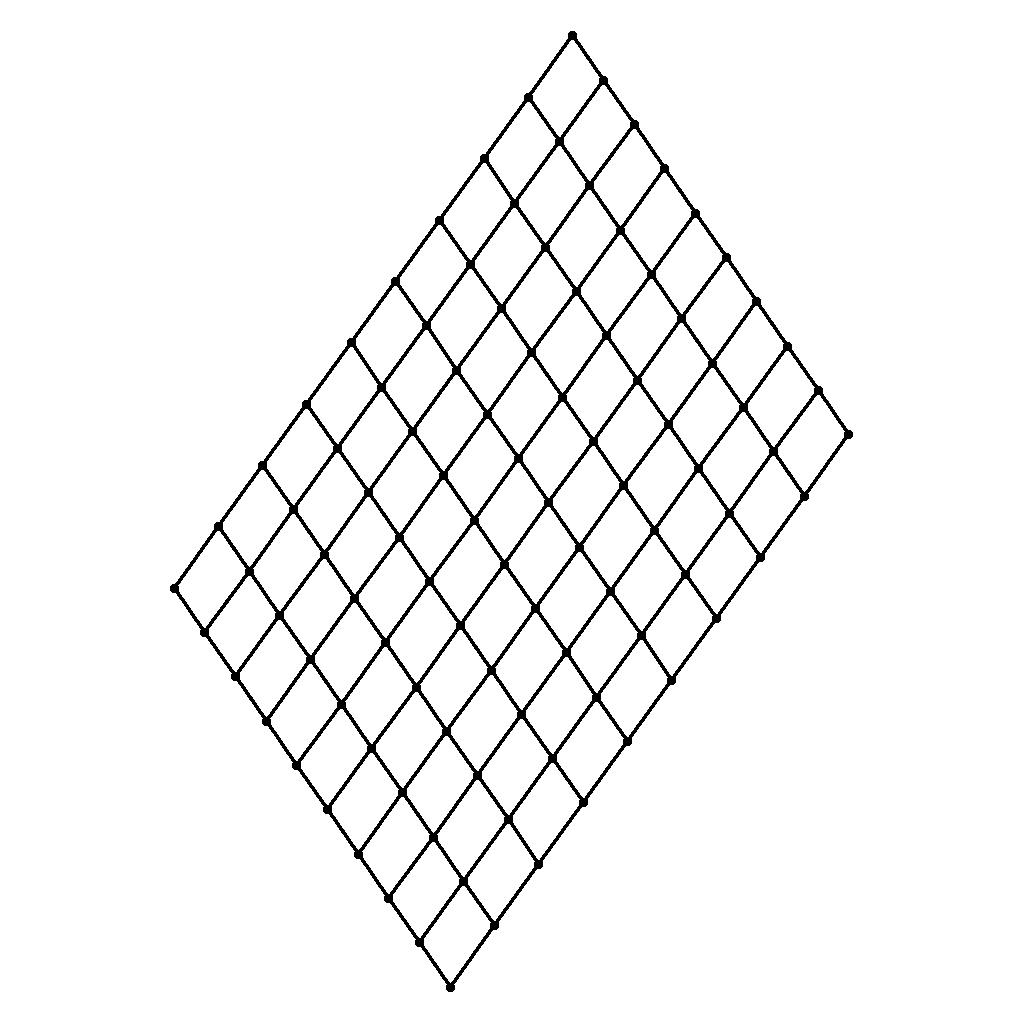
\includegraphics[width=\textwidth]{images/ima2.png}
\caption{Grille Transformée}
\label{fig:trlin_mesh}
\end{subfigure}
\caption{Transformation linéaire}\label{fig:trlin}
\end{figure}
A contrario, une application quelconque de $\R^2$ dans lui-même pourra donner des résultats notablement différents, tel  que celui présenté en figure \ref{fig:trnlin}
\begin{figure}[ht]
\centering
\begin{subfigure}[b]{0.45\textwidth}

\includegraphics[width=\textwidth]{images/ima1.png}
\caption{Grille initiale}
\label{fig:uni_mesh}
\end{subfigure}
\begin{subfigure}[b]{0.45\textwidth}
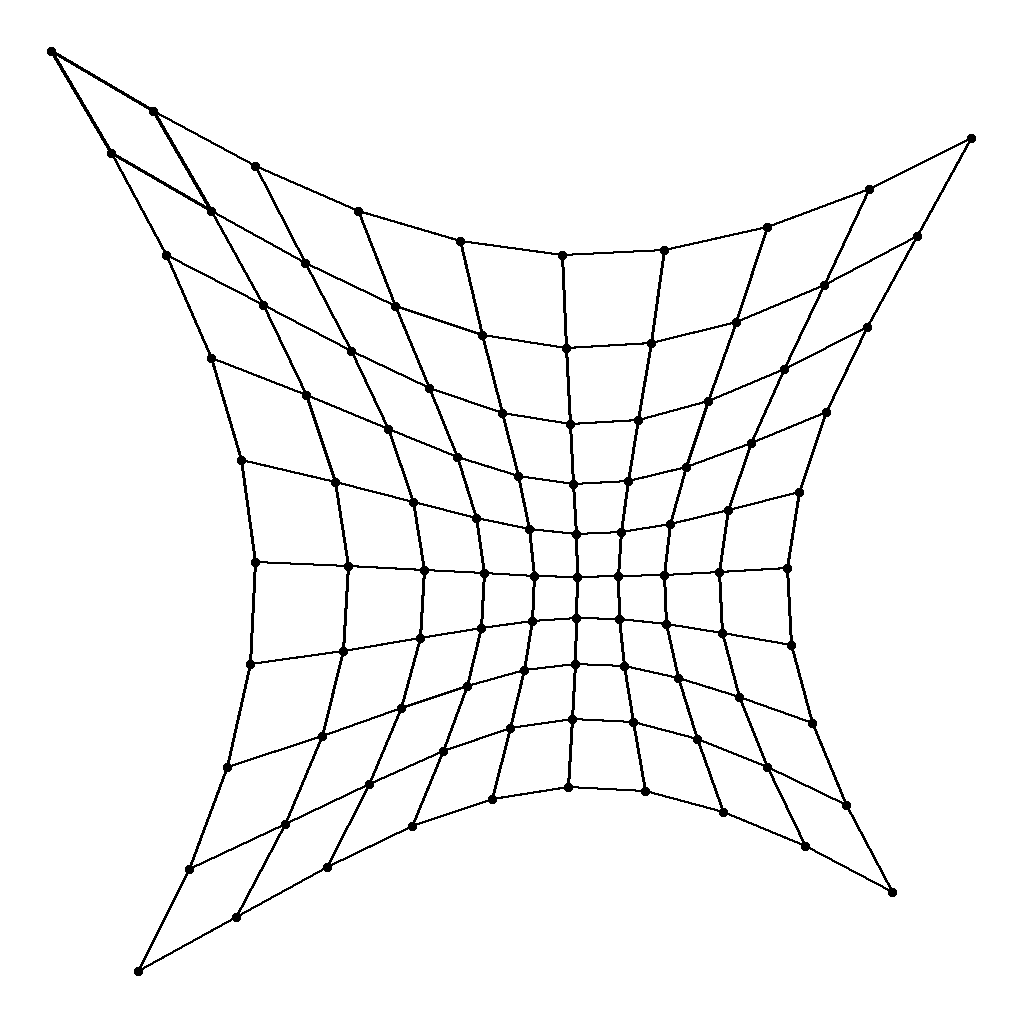
\includegraphics[width=\textwidth]{images/ima3.png}
\caption{Grille Transformée}
\label{fig:trnlin_mesh}
\end{subfigure}
\caption{Transformation non linéaire}\label{fig:trnlin}
\end{figure}

Dans le cas d'une application différentiable en un point, on peut d'une certaine façon faire coïncider localement la transformation non linéaire et l'endomorphisme qui lui est tangent en un point. Ceci est représenté sur la figure \ref{fig:diffapprox} où l'on remarque une très bonne coïncidence au voisinage du point où la différentielle est calculée.

\begin{figure}[ht]
\centering
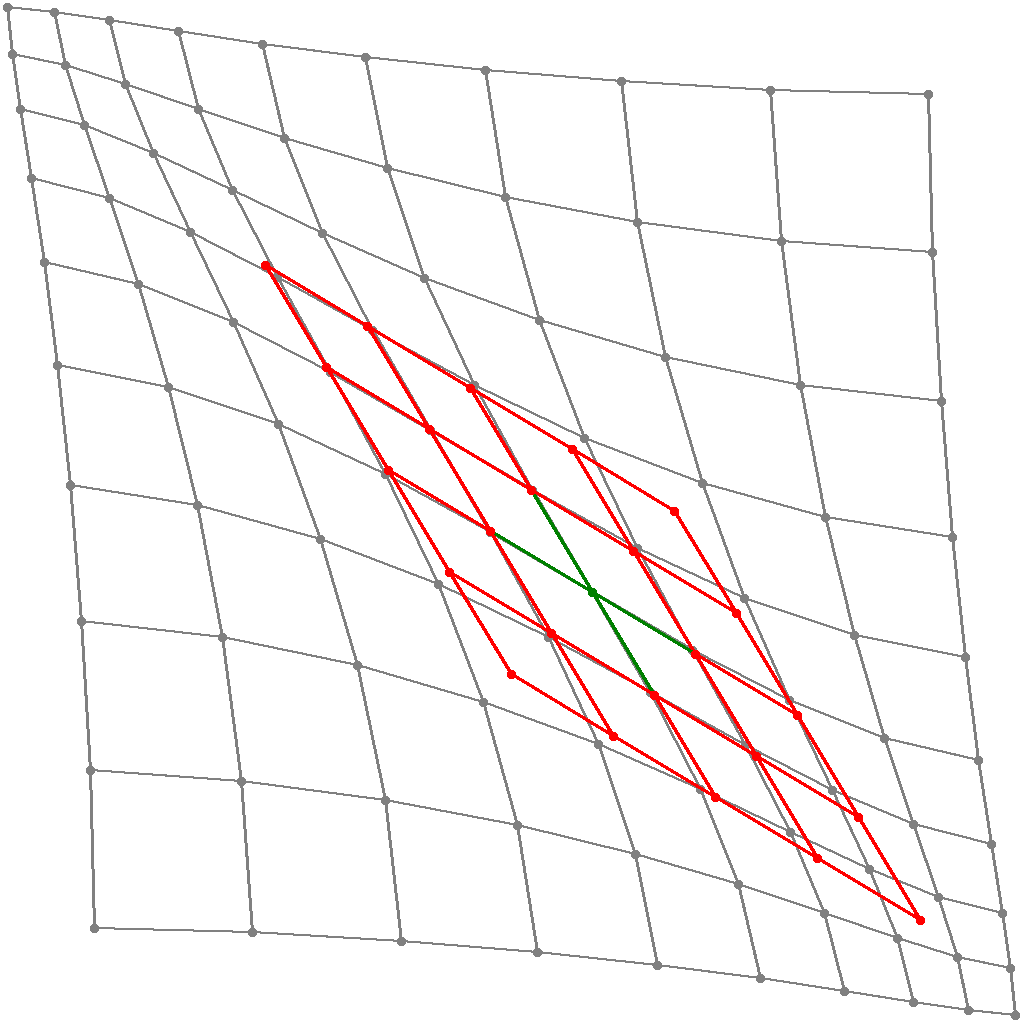
\includegraphics[width=0.5\textwidth]{images/ima4.png}
\caption{Approximation par une application affine}\label{fig:diffapprox}
\end{figure}

\subsection{Inversion locale}

Les propriétés de l'application linéaire tangente ne reflètent pas toujours celles de l'application initiale. On remarque qu'une application telle que $f \colon  x \in \R \mapsto x^3$ est inversible sur $\R$ tout entier, mais que sa dérivée en 0 est 0, donc non inversible. Pour obtenir une meilleure adéquation entre le comportement de l'application et de son modèle local, on imposera souvent une condition plus forte que la différentiabilité simple. 

\begin{fdefn}\label{def:strict_diff}
Soit $f \colon \Omega \to \R^2$. On dira que $f$ est strictement différentiable en $x_0 \in \Omega$ si l'on peut trouver un voisinage $V$ de $x_0$ et une application linéaire $H$ tels que:
\[
\forall (x,y) \in V^2, \, f(y) = f(x) + H(y-x) + o_{x_0}\left(\|y-x\|\right)
\]
\end{fdefn}

La différentiabilité stricte implique la différentiabilité simple, il suffit pour cela de considérer des couples de la forme $(x,x_0)$, mais la réciproque est fausse. L'intérêt majeur d'introduire cette notion réside dans le théorème suivant, dit d'inversion locale.

\begin{fthm}
Soit $f \colon \Omega \to \R^2$ une application strictement différentiable en $x_0 \in \Omega$. Si $f^\prime(x_0)$ est inversible, alors il existe un voisinage ouvert $U$ de $x_0$ et un voisinage ouvert $W$ de $f(x_0)$ tels que $f$ soit un homéomorphisme de $U$ sur $W$. De plus, $f^{-1}$ est strictement dérivable en $f(x_0)$ et on a $Df^{-1}(f(x_0)) = \left(f^{\prime}\right)^{-1}(x_0)$.
\end{fthm}
La preuve est très classique. Elle est détaillée ci-dessous en raison de son caractère constructif qui fournit un algorithme numérique permettant d'inverser en un point une application. Un résultat intermédiaire fondamental, le théorème du point fixe, va être maintenant rappelé en préliminaire à la preuve proprement dite.

\begin{fthm} \label{thm:pt_fixe}
Soit $E$ un espace de Banach (i.e. espace vectoriel normé complet pour la topologie induite par la norme). Soit $f$ une application de $E$ dans $E$ telle qu'il existe un réel $1 > k > 0$ vérifiant:
\[
\forall (x,y) \in E, \, \|f(x)-f(y)\| \leq k \|x-y\|
\]
alors il existe un unique $x_0 \in E$ tel que $f(x_0)=x_0$.
\end{fthm}
Une application vérifiant l'hypothèse de majoration ci-dessus est dite contractante. Il est important de bien noter que le réel $k$ doit être strictement inférieur à 1. 
\begin{proof}
Soit $x$ un point quelconque de $E$. On pose, pour tout entier $n$: $x_0 = x, x_{n+1}=f(x_n)$. Pour tout entier $n \geq 1$, on a:
\[
\left\| x_{n+1}-x_n \right \| = \left\| f(x_n)-f(x_{n-1}) \right \| \leq k \left\| x_n-x_{n-1} \right \|
\leq k^n \left\| x_1-x_0 \right \| 
\]
on en déduit que pour tout couple d'entiers $1 \leq p < q$:
\[
\left\| x_q - x_p \right \| \leq \sum_{i=p}^{q-1} \left\| x_{i+1} - x_i \right \| \leq \sum_{i=p}^{q-1} k^i \left\| x_1-x_0 \right \| \leq \frac{k^p}{1-k} \left\| x_1-x_0 \right \|
\]
Prouvant ainsi que la suite $(x_n)_{n \in \N}$ est de Cauchy. Comme $E$ est un espace complet, elle admet une limite $x^*$ dans $E$. $f$ est Lipschitzienne, donc continue. On a ainsi:
\[
x^* = \lim_{n \to +\infty } x_{n+1} = \lim_{n \to +\infty} f(x_n) = f\left( \lim_{n \to +\infty} x_n \right)
=f(x^*)
\]
montrant que $x^*$ est un point fixe de $f$. L'unicité s'obtient facilement en supposant l'existence de deux points fixes distincts $x^*, x^{*\prime}$. La majoration vérifiée par $f$ donne:
\[
\|x^* - x^{*\prime}\|= \|f(x^*) - f(x^{*\prime})\| \leq k \|x^* - x^{*\prime}\|
\] 
ce qui est impossible car $k < 1$.
\end{proof}
\begin{rem}
Le théorème du point fixe est remarquable sur deux points: 
\begin{itemize}
\item La convergence a lieu indépendamment du point de départ. 
\item La suite d'approximation du point fixe donne un algorithme explicite de calcul.
\end{itemize}
\end{rem}
On peut maintenant revenir à la preuve du théorème d'inversion locale qui sera elle aussi constructive.
\begin{proof}
L'idée principale est d'utiliser pour l'inversion le modèle linéaire fourni par la différentielle en $x_0$ en lieu et place de l'application $f$. 
Soit $V$ un voisinage de $x_0$ dans lequel l'application $f$ vérifie la condition de stricte différentiabilité:
\[
\forall (p,q) \in V, \, f(p)=f(q) +Df(x_0)(p-q) + o_{x_0}\left(\|p-q\|\right)
\]
 avec~:
 \[
  \left\|o_{x_0}\left(\|p-q\|\right)\right\| \leq \frac{\|Df(x_0)\|}{2} \|p-q\|
 \]
Soit $y \in f(V)$. On pose, pour tout $x \in V$:
\[
\Theta_y(x) = x + Df^{-1}(x_0)\left(y-f(x)\right)
\]
On notera que $\Theta_y$ modifie $x$ de telle façon que l'on aurait $y=f(\Theta_y(x))$ si $f$ était une application affine. On espère ici que le modèle linéaire donné par la différentielle sera suffisamment bon pour que $f(\Theta_y(x))$ soit plus proche de $y$ que ne l'était $x$. L'application $\Theta_y$ est contractante. Pour tout couple $(x,z)$ de points de $V$ on a:
\begin{align*}
\left\|\Theta_y(x) - \Theta_y(z)\right\| &  = \left\|z-x + Df^{-1}(x_0)\left(f(x)-f(z)\right) \right \| \\
& = \left\|Df^{-1}(x_0)\left( Df(x_0)(z-x) + f(x)-f(z)\right) \right \| \\
& \leq \|Df^{-1}(x_0)\|  \left\|o_{x_0}\left(\|z-x\|\right)\right\| \leq \frac{1}{2} \|z-x\|
\end{align*}
De plus, pour $x \in V$:
\begin{align*}
&\left\| \Theta_y(x) - x_0 \right \|  = \left \| x-x_0 + Df^{-1}(x_0)\left(y-f(x)\right) \right \| \\
& \leq \left \| x-x_0 + Df^{-1}(x_0)\left(f(x_0)-f(x) \right) \right \| + \left\| Df^{-1}(x_0)\left(y-f(x_0)\right)\right\| \\
& \leq \frac{\|x-x_0\|}{2} + \|Df^{-1}(x_0)\|\|y-f(x_0)\|
\end{align*}
d'où l'on déduit que si l'on choisi $x$ dans une boule $B(x_0,r) \subset V$, $\Theta_y(x)$ sera encore dans cette boule sous réserve que $y$ appartienne à la boule de centre $f(x_0)$ et de rayon $\eta=\|Df(x_0)\|r/2$. Sous ces conditions, le théorème du point fixe montre qu'il existe $z$ tel que $\Theta_y(z)=z$, qui équivaut à $f(z)=y$. En choisissant comme domaine de départ une boule ouverte $B(x_0,r\prime)$ contenue dans l'ouvert $B(x_0,r) \cap f^{-1}(B(f(x_0,\eta)))$, on assure que $f$ réalise une bijection sur $f(B(x_0,r\prime))$.

Soient $y,z$ deux points de $f(B(x_0,r\prime))$. En remarquant que:
\[
\Theta_y(f^{-1}(y))=f^{-1}(y), \Theta_z(f^{-1}(z))=f^{-1}(z)
\]
il vient:
\begin{align*}
& \|f^{-1}(y) - f^{-1}(z) \| \leq \\ &
\| \Theta_z(f^{-1}(z)) -\Theta_y(f^{-1}(z)) \| + \| \Theta_y(f^{-1}(z))-\Theta_y(f^{-1}(y)) \| \\
& \leq  \| \Theta_z(f^{-1}(z)) -\Theta_y(f^{-1}(z)) \|  + \frac{1}{2} \|f^{-1}(y) - f^{-1}(z) \|
\end{align*}
d où l'on tire:
\[
 \frac{1}{2} \|f^{-1}(y) - f^{-1}(z) \| \leq  \| \Theta_z(f^{-1}(z)) -\Theta_y(f^{-1}(z)) \| 
\]
Comme:
\[
\| \Theta_z(f^{-1}(z)) -\Theta_y(f^{-1}(z)) \|  = \| Df^{-1}(x_0) (z-y) \| \leq \| Df^{-1}(x_0)\| \|(z-y) \| 
\]
on a:
\[
 \|f^{-1}(y) - f^{-1}(z) \| \leq  2 \| Df^{-1}(x_0)\| \|(z-y) \| 
\]
prouvant le caractère lipschitzien de $f^{-1}$.

Enfin:
\begin{align*}
& \|f^{-1}(z)-f^{-1}(y) +Df^{-1}(x_0)(y-z)\| \leq \\
& \| Df^{-1}(x_0)\| \| y-z+Df(x_0)\left(
f^{-1}(z) - f^{-1}(y)\right) \|
\end{align*}
Le terme $y-z+Df(x_0)\left(f^{-1}(z) - f^{-1}(y)\right)$ est dans $o_{x_0}(\|f^{-1}(z)-f^{-1}(y)\|)$, mais aussi 
dans $o_{f(x_0)}(\|z-y\|)$, $f^{-1}$ étant lipschitzienne. On en déduit la stricte différentiabilité de $f^{-1}$, avec une différentielle en $f(x_0)$ égale à $Df^{-1}(x_0)$.
\end{proof}
\begin{rem}
Le théorème d'inversion locale est vrai dans le cadre beaucoup plus général des espaces de Banach.
\end{rem}

La proposition suivante permet d'utiliser le théorème d'inversion locale dans le cadre des applications de classe $C^1(\Omega)$, qui sont plus aisées à caractériser.
\begin{fprop}
Une application de classe $C^1(\Omega)$ est strictement différentiable en tout point de $\Omega$.
\end{fprop}
\begin{proof}
Soit $x_0\in \Omega$ et soit $\epsilon > 0$. Par continuité de $f^\prime$, il existe un voisinage $V_\epsilon$ de 
$x_0$ tel que pour tout $y$ dans $V_\epsilon$:
\[
\left\| f^{\prime}(y)-f^\prime(x_0) \right\| \leq \frac{\epsilon}{2} 
\]
Pour tout couple de points $(y,z)$ de $V_\epsilon$:
\begin{align*}
f(z)-f(y)-f^\prime(x_0)(z-y) & = \left(f(z)-f(y)-f^\prime(y)(z-y) \right)  \\
 & + \left(f^\prime(y)-f^\prime(x_0)\right)(z-y)
\end{align*}
Le premier terme du membre de droite est dans $o(\|z-y\|)$ en vertu de la différentiabilité de $f$ et quitte à réduire $V_\epsilon$, on peut supposer dans perte de généralité qu'il est majoré par $\epsilon \|z-y\| /2$. Le second terme est majoré par la même quantité, on a donc:
\[
\left\|f(z)-f(y)-f^\prime(x_0)(z-y)\right \| \leq  \epsilon \|z-y\|
\]
montrant la stricte différentiabilité de $f$ en $x_0$.
\end{proof}
La proposition précédente est locale: on peut supposer la différentiabilité au voisinage de $x_0$ et la continuité de $f^\prime$ en ce point pour assurer la strict différentiabilité en $x_0$.

On utilise le plus souvent dans le cadre $\R^2$ la proposition suivante pour montrer le caractère $C^1$ d'une application. 

\begin{fprop}
Soit $f \colon \Omega \to \R^2$. Si les dérivées partielles de $f$ existent et sont continues, alors $f$ est de classe $C^1(\Omega)$.
\end{fprop}
\begin{danger}
\begin{rem}
Attention, il s'agit d'une condition suffisante mais non nécessaire.
\end{rem}
\end{danger}

\subsection{Calcul numérique}
Le théorème d'inversion locale est constructif: il donne un algorithme explicite permettant d'approcher l'inverse d'une fonction point par point. On utilise très fréquemment cette remarquable propriété dans des applications de calcul numérique.
Nous présentons ici un code écrit en python réalisant l'implémentation informatique de ce qui vient d'être indiqué. Le code sera organisé autour d'une boucle dans laquelle seront exécutées les itérations du point fixe. Pour rester dans le cadre de ce cours, on se limitera aux cadre des applications de $\R^2$ dans $\R^2$, il est ainsi possible d'inverser directement les matrices jacobiennes. 

\begin{verbatim}
import math

# fonction à inverser
# x: vecteur de réels de taille 2
# return: vecteur de réels de taille 2
def my_func(x): 
    return [x[0]*x[0] + x[1]*x[1], x[0]*x[1]]
    
# matrice jacobienne de l'application à inverser
# x: vecteur de réels de taille 2
# return: matrice de réels de taille 2x2
def my_jac(x):
    return [[2 * x[0],2 * x[1]],[x[1],x[0]]]

# inversion d'une matrice 2x2
# une exception est levée lorsque la matrice est presque
# singulière à la precision machine
# a: matrice 2x2 de reels
# return: matrice 2x2  
def mat_inv(a):
    det = a[0][0] * a[1][1] - a[0][1] * a[1][0]
    if math.fabs(det) < 1e-8:
        # la matrice est presque singulière a la péecision machine
        # on lève une exception, au plus simple !
        raise ArithmeticError
    # inversion "à la main" de la matrice jacobienne
    return [[a[1][1]/det, -a[0][1]/det],[-a[1][0]/det, a[0][0]/det]]
    
# fonction réalisant une itération de point fixe 
# le premier argument représente le point où l'inverse
# est recherché.
# le second argument est le point candidat courant
# les arguments f,df representent respectivement la fonction
# à inverser et sa matrice jacobienne
# y: vecteur de réels de taille 2
# x: vecteur de réels de taille 2
# f: fonction à inverser
# ijac: inverse de la matrice jacobienne de la fonction
# à inverser au point de référence
# return: liste dont le premier &lement est un vecteur de 
# réels de taille 2, résultat de l'evaluation et le second
# argument est un réel donnant la norme de l'erreur commise.
def my_theta(y,x,f,ijac):
# évaluation de la fonction
    fx = f(x)
    # vecteur d'erreur 
    err=[y[0]-fx[0],y[1]-fx[1]]
    # terme correctif du modèle linéarisé
    a = ijac[0][0] * err[0] + ijac[0][1] * err[1]
    b = ijac[1][0] * err[0] + ijac[1][1] * err[1]
    # résultat final
    return [[x[0] + a, x[1] + b],math.sqrt(err[0] * err[0] + err[1] * err[1])]
    
# fonction réalisant une iteration de point fixe selon 
# la methode améliorée
# le premier argument représente le point ou l'inverse 
# est recherché.
# le second argument est le point candidat courant
# les arguments f,df representent respectivement 
# la fonction  à inverser et sa matrice jacobienne
# y: vecteur de reels de taille 2
# x: vecteur de reels de taille 2
# f: fonction à inverser
# df: jacobienne de la fonction a inverser
# return: liste dont le premier element est un vecteur de 
# réels de taille 2, résultat de l'evaluation 
# et le second argument est un réel donnant la norme
# de l'erreur commise.
def my_theta_i(y,x,f,df):
# évaluation de la fonction et de sa jacobienne
    fx = f(x)
    dfx = df(x)
    # inversion de dfx avec test de singularité
    idfx = mat_inv(dfx)           
    # vecteur d'erreur 
    err=[y[0]-fx[0],y[1]-fx[1]]
    # terme correctif du modele linéarisé
    a = idfx[0][0] * err[0] + idfx[0][1] * err[1]
    b = idfx[1][0] * err[0] + idfx[1][1] * err[1]
    # résultat final
    return [[x[0] + a, x[1] + b],math.sqrt(err[0] * err[0] + err[1] * err[1])]

# le code principal

# choix du type d'iteration

use_improved_iteration = False

# point de calcul initial, choisi hors des droites
#  y=x, y=-x sur lesquelles la matrice jacobienne 
# est singulière

x0 = [1.0, 2.0]

# point de référence pour l'application du théorème 
# d'inversion locale
# Il doit être assez proche de x0 pour que les itérations convergent

p = [1.2, 1.5]

# l'inverse du jacobien au point considéré

ijac = mat_inv(my_jac(p))

# la valeur image

y = my_func(x0)

# point de départ des itérations, toujours 
# hors des points singuliers

x=[2.0, 3.0]

# itération de point fixe jusqu'a éeduction suffisante de l'erreur

if use_improved_iteration:
    # itération améliorée
    res = my_theta_i(y, x, my_func, my_jac)
else:
    # itération standard
    res = my_theta(y, x, my_func, ijac)
while res[1] > 1e-8:
    # point courant = point de l'itération précédente
    x = res[0]
    # affichage du l'erreur et du point courant
    print(res[1],res[0])
    # nouvelle itération
    if use_improved_iteration:
        res = my_theta_i(y, x, my_func, my_jac)
    else:
        res = my_theta(y, x, my_func, ijac)
\end{verbatim}
On pourra facilement changer les valeurs des points de référence et de départ pour voir les différences de comportement du code.
Une méthode améliorée dans laquelle la valeur de la matrice jacobienne est recalculée à chaque itération est également disponible: il suffit pour cela de changer de \texttt{False} à \texttt{True} la valeur de la variable \texttt{use\_improved\_iteration}. Cet algorithme modifié est celui qui est employé en pratique. Il permet entre autres choses de retrouver des valeurs de paramètres inconnus à partir d'observations: il est ainsi possible en observant certains paramètres au cours d'un vol d'en déduire par exemple les coefficients aérodynamiques d'un avion. 
\vskip 12pt
\leftline{\textbf{Un peu d'histoire \dots}}
\vskip 12pt
\begin{tabular}{ll}
\multicolumn{2}{l}{\textbf{Gottfried Wilhelm von Leibniz}} \\[10pt]
\begin{minipage}{0.2\linewidth}
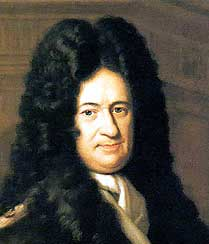
\includegraphics[scale=0.3]{images/Gottfried_Wilhelm_von_Leibniz.jpg}
\end{minipage}
&
\begin{minipage}{0.65\linewidth}
Né le  1 juillet 1646 à Liepzig, mort le 14 novembre 1716 à Hanovre, Gottfried Liebniz est un esprit universel,
philosophe, mathématicien, logicien, juriste et diplomate. Il partage avec Isaac Newton la paternité du calcul différentiel et intégral, une controverse sur l'antériorité de la découverte ayant opposé les deux hommes. La notation de Liebniz $\partial f$ est celle qui a été retenue par les mathématiciens, de même que le symbole $\int$ pour l'intégrale.
\end{minipage}\\
\multicolumn{2}{l}{\textbf{Isaac Newton}} \\[10pt]
\begin{minipage}{0.2\linewidth}

\includegraphics[scale=0.3]{images/isaac_newton.jpg}
\end{minipage}
& 
\begin{minipage}{0.65\linewidth}
Né le  4 janvier 1643 à Woolsthorpe, mort le 31 mars 1727 à Kensington est un scientifique et philosophe anglais surtout connu pour sa loi de la gravitation universelle. Il a apporté de nombreuses contributions dans le domaine des mathématiques, en particulier la formule du binôme et l'algorithme de recherche des zéros d'une fonction qui porte son nom. Ses travaux sur le calcul infinitésimal on été publiés postérieurement à ceux de Liebniz ce qui a donné lieu à son époque à une dispute sur l'attribution de cette découverte. On lui doit également de nombreux travaux en optique.
\end{minipage}\\
\multicolumn{2}{l}{\textbf{Stefan Banach}} \\[10pt]
\begin{minipage}{0.2\linewidth}
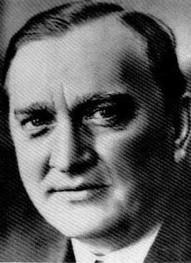
\includegraphics[scale=0.3]{images/banach.jpg}
\end{minipage}
& 
\begin{minipage}{0.65\linewidth}
Né le 30 mars 1892 à Ostrowsko, mort le 31 août 1945 à Lviv. Banach est un mathématicien fécond, fondateur de l'analyse fonctionnelle. Ses travaux sur les espaces vectoriels topologiques le conduisent à définir les espaces qui portent maintenant son nom. On lui doit également le théorème du point fixe pour les applications contractantes, ainsi que le célèbre paradoxe de Banach-Tarski.
\end{minipage}
\end{tabular}

\section{L'espace vectoriel des nombres complexes}
L'étude des propriétés des applications de $\C$ dans $\C$ est un domaine particulièrement fécond des mathématiques qui a conduit à de très nombreux résultats en analyse. Les remarquables propriétés différentielles de ces applications en ont popularisé l'usage bien au delà du cadre des mathématiques. Dans toutes les applications de physique demandant la résolution d'équations de type Poisson, les techniques issues de la théorie des fonctions de la variable complexe étaient les méthodes de choix jusqu'à l'avènement des calculateurs électroniques. On les utilise encore aujourd'hui lorsque l'on souhaite une expression analytique de la solution, ou tout simplement pour la simplicité et l'élégance.  

L'ensemble $\C$ des nom\-bres complexes possède deux structures naturelles d'espace vectoriel, l'une d'espace vectoriel complexe et l'autre d'espace vectoriel réel. $\C$ considéré comme espace vectoriel sur lui-même est de dimension $1$ alors qu'il est de dimension 2 en tant qu'espace réel. Dans de dernier cas, il est isomorphe à $\R^2$ par l'isomorphisme canonique $(x,y) \in \R^2 \mapsto x + i y$. Pour un complexe $z=x+iy$, on rappelle que le point $(x,y)$ est appelé \textbf{affixe} de $z$.

Soit $f : \Omega \subset \mathbb{C} \to \mathbb{C}$ une fonction de la variable complexe. En posant $z = x + iy$, on peut écrire~:
\[
f(z) = P(x,y) + i Q(x,y)
\]
avec $P$ et $Q$ les parties réelle et imaginaire de $f$. On peut par cette décomposition associer à l'application initiale $f$ une application de $\R^2$ dans $\R^2$ que l'on continuera à noter $f$:
\[
f \colon (x,y) \mapsto \left(P(x,y), Q(x,y)\right)
\]
Dans la suite, on passera librement d'une notation à une autre en fonction du contexte. 

Muni de la norme induite par la norme euclidienne de $\mathbb{R}^2$,
$\mathbb{C}$ est un espace de Banach réel. La norme d'un nombre
complexe $z$ est appelée \textbf{module} de $z$, noté $|z|$.
Le module est aussi une norme sur $\C$ considéré comme espace vectoriel sur lui-même. 

\begin{rem}
Le produit usuel de deux nombres complexes fait de $ \mathbb{C}$ une
algèbre sur lui-même. La relation $\forall (z_1,z_2) \in \mathbb{C}^2,
|z_1 z_2| = |z_1||z_2|$ montre que l'algèbre en question est
normée. Comme $\mathbb{C}$ est aussi un espace de Banach pour la norme
$|.|$, on dit qu'il s'agit d'une algèbre de Banach.
\end{rem}
Il est important de noter que la distinction entre $\mathbb{C}$ considéré comme
$\mathbb{R}$-espace vectoriel et $\mathbb{C}$-espace vectoriel a une conséquence
fondamentale sur les applications linéaires qui ont pour domaine l'un ou l'autre
de ces espaces.
\begin{fprop}
Soit $f \colon \mathbb{C} \to \mathbb{C}$ une application $\mathbb{C}$-linéaire.
Il existe un complexe $\lambda \in \mathbb{C}$ tel que pour tout $z \in
\mathbb{C}$, $f(z) = \lambda z$
\end{fprop}
\begin{proof}
La preuve est plus courte que l'énoncé. Si $f$ est $\mathbb{C}$-linéaire, pour
tout $z \in \mathbb{C}$, $f(z) = f(z.1)= z f(1)$ et le $\lambda$ recherché est
donc $f(1)$.
\end{proof}
\begin{fdefn}
Soit $f \colon \mathbb{C} \to \mathbb{C}$. On dit que $f$ est $\mathbb{C}$-anti
linéaire si pour tout $(\lambda,z_1,z_2) \in \mathbb{C}^3$, on a:
\[
f(\lambda z_1 + z_2) = \overline{\lambda} f(z_1) + f(z_2)
\]
\end{fdefn}
De même que pour les applications $\mathbb{C}$-linéaires, toute application $f$
qui est $\mathbb{C}$-anti linéaire admet une écriture:
\[
z \mapsto f(z) = \lambda \overline{z}
\]
avec comme précédemment $\lambda = f(1)$.
\begin{fprop}\label{prop:dec_lin}
Soit $f \colon \mathbb{C} \to \mathbb{C}$ une application 
$\mathbb{R}$-linéaire. Il existe une unique application $\mathbb{C}$-linéaire
$g$ et une unique application $\mathbb{C}$-anti linéaire $h$ telles que $f = g
+ h$.
\end{fprop}
\begin{proof}
Pour tout $z=x + i y \in \mathbb{C}$, la $\mathbb{R}$-linéarité montre que:
\[
f(z) = f(x + iy) = x f(1) + y f(i)
\]
Par ailleurs:
\[
x = \frac{z + \overline{z}}{2}, \; y = -i \frac{z - \overline{z}}{2}
\]
En regroupant les termes:
\[
f(z) = z \left(\frac{f(1)-if(i)}{2}\right) + \overline{z}
\left(\frac{f(1)+if(i)}{2}\right)
\]
soit:
\[
g \colon z \mapsto  z \left(\frac{f(1)-if(i)}{2}\right) \; h \colon z \mapsto \overline{z}
\left(\frac{f(1)+if(i)}{2}\right)
\]
\end{proof}
Bien que d'apparence anodine, cette proposition sera fondamentale pour la notion
de dérivabilité dans $\mathbb{C}$. En effet, il est relativement facile de
tester qu'une application $f \colon \mathbb{C} \to \mathbb{C}$ est
différentiable en un point si $\mathbb{C}$ est considéré comme espace vectoriel
réel: on est en effet dans ce cas ramené à une application de $\mathbb{R}^2$ dans  $\mathbb{R}^2$. La différentielle en un point d'une telle application est
$\mathbb{R}$-linéaire et, en vertu du résultat précédent, ne pourra être
$\mathbb{C}$-linéaire que si le terme $\mathbb{C}$-anti linéaire s'annule, ce
qui conduira aux conditions de Cauchy pour la différentiabilité dans
$\mathbb{C}$.


\begin{fdefn}
Soit $f : \Omega \to \mathbb{C}$ avec $\Omega$ ouvert de $\C$ et $z_0 \in \Omega$.
On dira que $f$ a pour limite $l$ au point $z_0$ si~:
\[
\forall \epsilon > 0, \exists \eta > 0 \mbox{ tel que } |z-z_0| < \eta \Rightarrow
|f(z)-l| < \epsilon 
\]
\end{fdefn}
Comme dans le cas réel, $f$ sera dite continue au point $z_0$ si sa
limite est $f(z_0)$ en ce point ou si $z_0$ est un point isolé (on
rappelle qu'un point est dit isolé si la partie réduite à ce point est
ouverte).
\begin{fdefn}
On appelle $\mathbb{C}$ achevé l'ensemble $\overline{\mathbb{C}} = \mathbb{C} \cup \omega$
muni de la topologie dont les ouverts sont d'une part les ouverts de
$\mathbb{C}$ et d'autre part les complémentaires dans
$\overline{\mathbb{C}}$ des compacts de $\mathbb{C}$.
\end{fdefn}

On attribue à $\omega$, dit point à l'infini, les propriétés
suivantes~:
\begin{itemize}
\item $\forall \epsilon \in \mathbb{R},  |\omega| > \epsilon$.
\item $\omega \omega = \omega$.
\item $\forall z \neq 0 \in \mathbb{C}, z \omega = \omega, z / \omega
  = 0, \omega /z  = \omega$
\end{itemize}

Une base de voisinages de $\omega$ s'obtient en considérant les
ensembles~:
\[
B(\omega,r) = \{ z \in   \overline{\mathbb{C}}, |z| > r \}
\]
avec $r$ réel strictement positif.
Un voisinage de $\omega$ est une partie de $\overline{\mathbb{C}}$
contenant un ensemble $B(\omega, r)$.
\begin{fdefn}
Soit $f : \mathbb{C} \to \mathbb{C}$. On dira que $f$ a pour limite
$l$ à l'infini si~:
\[
\forall \epsilon > 0, \exists \eta > 0 \mbox { tel que } |z| > \eta
\Rightarrow |f(z) -l| < \epsilon
\]
\end{fdefn}
Si $f$ admet une limite à l'infini, on peut la prolonger par
continuité sur $\overline{\mathbb{C}}$ en posant $f(\omega) =l$.
$\overline{C}$ est difféomorphe à la boule unité $\mathbb{S}^2$ de $\R^3$. On peut facilement s'en convaincre en utilisant l'application suivant, appelée projection stéréographique:
\[
\begin{cases}
(x,y,z) \in \mathbb{S}^2-\{(0,0,1)\} \mapsto \frac{x}{1-z} + i \frac{y}{1-z} \\
(0,0 ,1) \mapsto \omega
\end{cases}
\]

On utilisera fréquemment dans la suite des propriétés liées à la connexité. Afin
de simplifier les énoncés, on introduit la définition suivante:
\begin{fdefn}
Un domaine $\Omega \subset \mathbb{C}$ est un ouvert connexe non vide de
$\mathbb{C}$
\end{fdefn}

\section{Holomorphie}
\begin{fdefn}
Soit $\Omega $ un ouvert de $\mathbb{C}$ et soit $f : \Omega \to
\mathbb{C}$. On dira que $f$ est holomorphe en $z_0 \in \Omega$ si
l'application~:
\[
z \Omega \to \frac{f(z) - f(z_0)}{z - z_0}
\]
admet une limite en $z_0$.
\end{fdefn}
\begin{rem}
Une application holomorphe en un point est aussi dite dérivable en ce
point. On note généralement la limite de l'application ci-dessus par
$f^\prime(z_0)$.
\end{rem}
\begin{fprop}\label{prop:hol_1}
Pour que $f$ soit holomorphe en $z_0$, il faut et il suffit que~:
\begin{itemize}
\item $f$ soit différentiable en $z_0$ en tant qu'application d'un
  ouvert de $\mathbb{R}^2$ dans $\mathbb{R}^2$.
\item Les parties réelles et imaginaires $P,Q$ de $f$ vérifient les
  conditions de Cauchy~:
\begin{align*}
&\frac{\partial P}{\partial x} = \frac{\partial Q}{\partial y} \\
&\frac{\partial P}{\partial y} = - \frac{\partial Q}{\partial x}
\end{align*}
\end{itemize}
\end{fprop}
\begin{proof}
La dérivabilité en $z_0$ s'écrit aussi, pour $z \in V$ avec $V$ voisinage ouvert de $z_0$~:
\[
f(z) = f(z_0) +(z-z_0)f^\prime(z_0) + o(|z_0|)
\]
soit encore, en utilisant les parties réelles et imaginaires $P,Q$ et en posant $z=x+iy, z_0 = x_0 + i y_0$~:
\begin{align*}
\left (
\begin{array}{l}
P(x,y) \\
Q(x,y)
\end{array}
\right ) = &
\left (
\begin{array}{l}
P(x_0,y_0) \\
Q(x_0,y_0)
\end{array}
\right )
+ \\
&\left (
\begin{array}{ll}
\mathcal{R}(f^\prime(z_0)) & -\mathcal{I}(f^\prime(z_0)) \\
\mathcal{I}(f^\prime(z_0)) & \mathcal{R}(f^\prime(z_0)) \\
\end{array}
\right )
\left (
\begin{array}{l}
x-x_0 \\
y-y_0
\end{array}
\right ) +
o(|z-z_0|)
\end{align*}
Cette expression exprime la différentiabilité de $f$ en tant
qu'application d'une partie de $\mathbb{R}^2$ dans $\mathbb{R}^2$,
l'application dérivée étant l'application linéaire de matrice
représentative~:
\[
\left (
\begin{array}{ll}
\mathcal{R}(f^\prime(z_0)) & -\mathcal{I}(f^\prime(z_0)) \\
\mathcal{I}(f^\prime(z_0)) & \mathcal{R}(f^\prime(z_0)) \\
\end{array}
\right )
\]
mais par ailleurs, cette matrice doit aussi avoir comme expression~:
\[
\left (
\begin{array}{ll}
\frac{\partial P}{\partial x} & \frac{\partial P}{\partial y} \\
\frac{\partial Q}{\partial x} & \frac{\partial Q}{\partial y} \\
\end{array}
\right )
\]
associé au résultat précédent, on obtient les conditions de Cauchy~:
\begin{align*}
&\frac{\partial P}{\partial x} = \frac{\partial Q}{\partial y} \\
&\frac{\partial P}{\partial y} = - \frac{\partial Q}{\partial x}
\end{align*}
L'équivalence entre holomorphie et différentiabilité au sens de
$\mathbb{R}^2$ avec conditions de Cauchy est alors immédiate.
\end{proof}

\begin{fdefn}
Une application holomorphe en tout point d'un domaine $\Omega$ est
dite holomorphe dans ce domaine.
\end{fdefn}

La définition de la différentiabilité en $(x_0,y_0)$ de l'application
$f$ considérée de $\mathbb{R}^2$ dans $\mathbb{R}^2$, s'écrit de façon
générale~: 
\[
f(x,y) = f(x_0,y_0) + f^\prime(x_0,y_0) \left ( \begin{array}{c} x-x_0 \\ y-y_0 \end{array} \right )
+o \left ( \left \|  \begin{array}{c} x-x_0 \\ y-y_0 \end{array} \right \| \right )
\]
en écrivant~:
\[
x = \frac{z+\overline{z}}{2} \, , \, y = \frac{z-\overline{z}}{2i}
\]
il vient, après développement et passage dans $\mathbb{C}$~:
\begin{align*}
f(z) = f(z_0) &+ \frac{z-z_0}{2} 
\left (
\frac{\partial P}{\partial x} + \frac{\partial Q}{\partial y} - i 
\frac{\partial P}{\partial y} + i \frac{\partial Q}{\partial x}
\right ) \\&+
\frac{\overline{z}-\overline{z_0}}{2} 
\left (
\frac{\partial P}{\partial x} - \frac{\partial Q}{\partial y} + i 
\frac{\partial P}{\partial y} + i \frac{\partial Q}{\partial x}
\right ) + o(|z-z_0|)
\end{align*}
Le membre de droite de l'égalité est formé d'une partie $\mathbb{C}$-linéaire et
d'une partie $\mathbb{C}$-anti linéaire qui correspond à la décomposition de la
différentielle de $f$, considérée comme application de $\mathbb{R}^2$ dans
$\mathbb{R}^2$, en application du résultat de la proposition \ref{prop:dec_lin}.
On posera:
\begin{align*}
&\frac{\partial f}{\partial z} = \frac{1}{2} \left (\frac{\partial P}{\partial x} + \frac{\partial
Q}{\partial y} - i \frac{\partial P}{\partial y} + i \frac{\partial Q}{\partial x} \right) \\
& \frac{\partial f}{\partial \overline{z}} = \frac{1}{2} \left (\frac{\partial P}{\partial x} -
\frac{\partial Q}{\partial y} + i
\frac{\partial P}{\partial y} + i \frac{\partial Q}{\partial x}
\right)
\end{align*}
Soit:
\[
f(z)=f(z_0)+\frac{\partial f(z_0)}{\partial z}(z-z_0)+\frac{\partial
f(z_0)}{\partial \overline{z}}(\overline{z}-\overline{z_0})+o(|z-z_0|)
\]
On remarque alors que les conditions de Cauchy prennent la forme synthétique~:
\[
\left . \frac{\partial f }{\partial \overline{z}} \right |_{z = z_0} = 0
\]
Ce qui permet une reformulation de la proposition \ref{prop:hol_1}:
\begin{fprop}
Pour que $f$ soit holomorphe en $z_0$, il faut et il suffit que $f$ soit différentiable en $z_0$ en tant qu'application d'un
  ouvert de $\mathbb{R}^2$ dans $\mathbb{R}^2$ et que:
\[
\left . \frac{\partial f }{\partial \overline{z}} \right |_{z = z_0} = 0
\]
Sous ces conditions on a alors:
\[
f^\prime(z_0) = \left . \frac{\partial f }{\partial z} \right |_{z = z_0} 
\]
\end{fprop}

Dans certains cas, il est nettement
plus simple de vérifier les conditions d'holomorphie à partir de cette forme: il
suffit en effet de considérer dans l'expression de $f$ les variables
$z,\overline{z}$ comme indépendantes et de calculer les dérivées partielles
correspondantes: si le terme anti-linéaire est nul, la dérivée partielle par
rapport à $z$ donne directement $f^\prime(z_0)$.

Soit $f$ une fonction de $\mathbb{R}^2 \to \mathbb{R}^2$. On dira que
$f$ est de classe $C^2$ dans un domaine  $\Omega \subset \mathbb{R}^2$
si ses dérivées partielles secondes existent et sont continues dans
$\Omega$. On dira que $f$ de classe $C^2$ est harmonique dans $\Omega$ si~:
\[
\forall (x,y) \in \Omega, \, \left . \frac{\partial^2 f}{\partial x^2}
\right |_{(x,y)} + \left . \frac{\partial^2 f}{\partial y^2} \right
|_{(x,y)} = 0 
\]

Si une application $f$ de la variable complexe, dont les parties
réelles et imaginaires sont de classe $C^2$, est holomorphe dans un
domaine $\Omega$, les parties réelles et imaginaires sont harmoniques
dans $\Omega$. Cette proposition admet une réciproque~:
\begin{theorem}
Soit $P$ une application de classe $C^2$ dans un domaine étoilé
$\Omega$ de
$\mathbb{R}^2$. 
Si $P$ est harmonique, il existe une application $f$ holomorphe dans $\Omega$ et
admettant $P$ pour partie réelle.
\end{theorem}
\begin{proof}
L'application $f$ recherchée sera de la forme~:
$f = P + i Q$, différentiable en tout point de $\Omega$ et vérifiant
les conditions de Cauchy. On pose~:
\[
\omega = - \frac{\partial P}{\partial y} dx + \frac{\partial P}{\partial
  x} dy
\]
on a:
\[
d \omega = \left(\frac{\partial^2 P}{\partial x^2} + \frac{\partial^2
P}{\partial y^2} \right)dx \wedge dy 
\]
Par hypothèse on a~:
\[
\frac{\partial^2 P}{\partial x^2} + \frac{\partial^2 P}{\partial y^2} = 0  
\]
on en déduite que $d\omega=0$. L'ouvert $\Omega$ étant étoilé, le théorème de Poincaré
permet d'affirmer l'existence d'une application $Q$ (forme de degré 0, définie
à une constante additive près) telle que $\omega = d Q$.
En identifiant les expressions de $\omega$, on vérifie les conditions de Cauchy:
\[
\frac{\partial P}{\partial x} = \frac{\partial Q}{\partial y} ,\quad
\frac{\partial P}{\partial y} = - \frac{\partial Q}{\partial x}
\]
montrant que $Q$ est bien la partie imaginaire recherchée.

\end{proof}
\begin{rem}
Le théorème précédent reste vrai avec des hypothèses plus larges sur l'ouvert $\Omega$. 
\end{rem}
La plupart des propriétés usuelles de la dérivation des fonctions de
la variable réelle passent au cas complexe. En particulier on a~:
\begin{fprop}
\begin{itemize}
\item Linéarité. Si $f,g$ sont holomorphes en $z_0$, toute
  combinaison linéaire à coefficients complexes de $f$ et de $g$ est
  encore holomorphe en $z_0$ et l'on a, pour $ a,b \in \mathbb{C}$, 
$(a f + b g)^\prime = a f^\prime + b g^\prime$.
\item Produit. Soient $f,g$ holomorphes en $z_0$, le produit $fg$ est
  holomorphe en $z_0$ et $(fg)^\prime |_{z_0} = f(z_0)^\prime g(z_0) + f(z_0) g^\prime(z_0)$.
\item Quotient. Soient $f,g$ holomorphes en $z_0$ avec $g(z_0)
  \neq 0$. L'application $f/g$ est holomorphe en $z_0$ avec~:
\[
\left .\left ( \frac{f}{g} \right )^\prime \right |_{z_0}  = \frac{f^\prime(z_0) g(z_0) - f(z_0) g^\prime(z_0)}{g^2(z_0)}
\]
\item Composition. Soit $f$ holomorphe dans un domaine $\Omega$ et
  soit $g$ holomorphe dans $\Omega^\prime$ avec $f(\Omega) \subset
  \Omega^\prime$. L'application $g \circ f$ est holomorphe dans
  $\Omega$ et l'on a~:
\[
(g \circ f )^\prime (z) = f^\prime (z) g^\prime (f(z)) \, , \, \forall
z \in \Omega
\]
\item Soit $f$ holomorphe dans un domaine $\Omega$ et bijective, et
  soit $f^{-1}$ son application réciproque. $f^{-1}$ est holomorphe
  dans $f(\Omega)$ et~:
\[
\forall z \in f(\Omega), \, (f^{-1})^\prime(z) = \frac{1}{f^\prime (f^{-1}(z))}
\]
\end{itemize}
\end{fprop}
Pour la dernière propriété, on notera que si $f=P+iQ$ est holomorphe, la matrice
de son application dérivée (en tant qu'application de $\mathbb{R}^2$ dans $\mathbb{R}^2$)
est~:
\[
\left (
\begin{array}{cc}
\frac{\partial P}{\partial x} & \frac{\partial Q}{\partial x} \\
\frac{\partial P}{\partial y} & \frac{\partial Q}{\partial y} \\
\end{array}
\right )
\]
Soit encore, avec les conditions de Cauchy,
\[
\left (
\begin{array}{cc}
\frac{\partial P}{\partial x} & -\frac{\partial P}{\partial y} \\
\frac{\partial P}{\partial y} & \frac{\partial P}{\partial x} \\
\end{array}
\right )
\]
dont le déterminant vaut~:
\[
\frac{\partial P}{\partial x}^2 + \frac{\partial P}{\partial y}^2 =
|f^\prime(x+iy)|^2 
\]
On en déduit que dans la règle de dérivation de l'application
réciproque, la condition $f^\prime(f^{-1}) \neq 0$ est automatiquement
vérifiée pour tout $z \in \Omega$, $f$ étant bijective holomorphe,
donc d'application linéaire tangente (de $\mathbb{R}^2$ dans
$\mathbb{R}^2$) inversible en tout point.


\begin{exercice}
Soit $\Omega$ un domaine non vide de $\mathbb{C}$ et soit $f$ application
holomorphe sur $\Omega$. Montrer que les conditions suivantes sont équivalentes~:
\renewcommand{\theenumi}{\alph{enumi}}
\begin{enumerate}
\item $f$ est constante sur $\Omega$.
\item $\Re(f)$ est constante sur $\Omega$.
\item $\Im(f)$ est constante sur $\Omega$.
\item $|f|$ est constante sur $\Omega$.
\end{enumerate}
\end{exercice}
\section{Transformations conformes}
Soit $f$ une application holomorphe dans un domaine $\Omega$ de
$\mathbb{C}$ et soient deux chemins différentiables $\gamma_1,
\gamma_2 : [0,1] \to \Omega$ tels qu'il existe $t_0 \in  [0,1]$ pour
lequel $\gamma_1(t_0) = \gamma_2(t_0)$. L'application $f \circ
\gamma_1$ (resp. $f \circ \gamma_2$ ) est différentiable sur
$[0,1]$. 
En $t_0$ on obtient~:
\[
(f \circ \gamma_1)^\prime (t_0) = f^\prime (z_0) \gamma_1^\prime (t_0) 
\]
\[
(f \circ \gamma_2)^\prime (t_0) = f^\prime (z_0) \gamma_2^\prime (t_0) 
\]
avec $z_0 = \gamma_1(t_0) = \gamma_2(t_0)$ et  $f^\prime(z_0)$ la matrice
de l'application linéaire tangente à $f$ en $z_0$.
Le produit scalaire $ \langle f \circ \gamma_1)^\prime (t_0),(f \circ
\gamma_2)^\prime (t_0) \rangle $ vaut $\langle  f^\prime (z_0)
\gamma_1^\prime (t_0) ,  f^\prime (z_0) \gamma_2^\prime (t_0) \rangle
$, soit  $\langle  f^{\prime t} (z_0)  f^\prime(z_0) \gamma_1^\prime
(t_0), \gamma_2^\prime (t_0) \rangle$. Un calcul simple montre que~:
\[
 f^{\prime t} (z_0)  f^\prime(z_0) = \left (
\begin{array}{cc}
|\frac{\partial f}{\partial z}(z_0)|^2 & 0 \\
0 & |\frac{\partial f}{\partial z}(z_0)|^2 \\
\end{array}
\right )
\]
L'angle entre les vecteurs $ (f \circ \gamma_1)^\prime (t_0)$ et $ (f
\circ \gamma_2)^\prime (t_0) $ sera donc le même que celui entre
$\gamma_1^\prime (t_0)$ et $ \gamma_2^\prime (t_0)$. Une
transformation de $\mathbb{R}^2 \to \mathbb{R}^2$ préservant les
angles entre vecteurs tangents à deux chemins est appelée conforme. En
vertu du résultat précédent, on peut associer une transformation
conforme à une application holomorphe dans un domaine.

\begin{figure}[h]
\scalebox{.5}{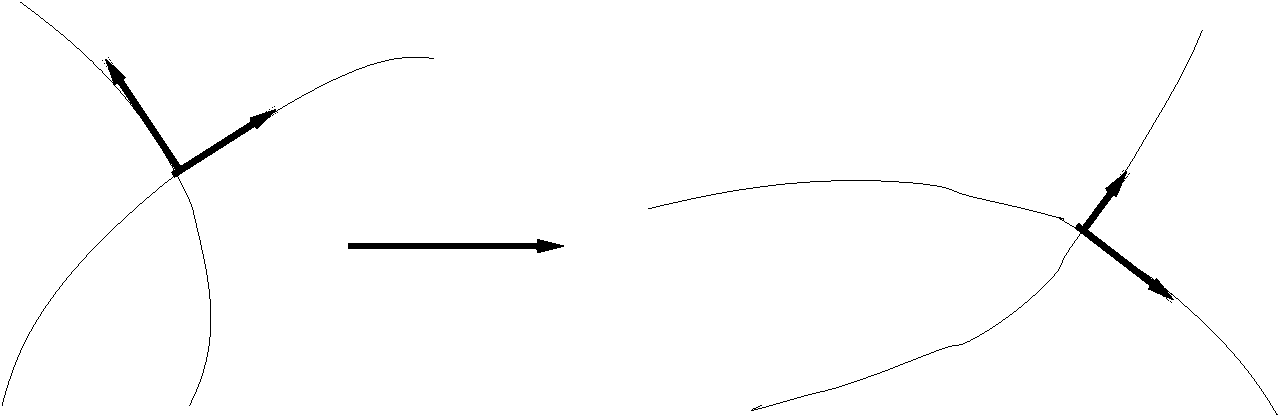
\includegraphics{images/trans_conforme.pdf}}
\caption{Transformation conforme}\label{Fi:fig2}
\end{figure}

Soit $f = P + i Q$ holomorphe dans un domaine $\Omega$. On considère
les familles de courbes définies par les équations implicites $P = t$,
$Q = u$ avec $t,u$ réels. Ces deux famille de courbes sont
orthogonales ; en effet, si l'on considère leurs images par la
transformation conforme associée à $f$, on obtient les courbes $x = t$
et $y = u$ qui sont orthogonales. Par ailleurs, les parties réelles et
imaginaires de $f$ sont des application harmoniques, i.e. solutions de
l'équation $\Delta P = 0$ (resp. $\Delta Q = 0$) avec $\Delta$
opérateur laplacien. De nombreuses relations physiques se traduisent
par une équation de la forme précédente~: c'est en particulier le cas
pour les écoulements de fluides incompressibles ou pour le potentiel
électrique. Pour résoudre ces problèmes physiques, l'utilisation de
transformations conformes associées à des application holomorphes est
souvent la méthode la plus simple. 
Soit à trouver une application $u$ de classe $C^2$ dans un domaine
$\Omega \subset \mathbb{R}^2$ de bord régulier $\partial \Omega$ telle que ~:
\[
\left \{
\begin{array}{cc}
\Delta u = 0 & \mbox{ dans } \Omega \\
u = g & \mbox{ sur } \partial \Omega \\
\end{array}
\right .
\] 
avec $g$ de classe $C^2$ sur $\partial \Omega$. S'il existe une
application holomorphe $f = P + i Q$ telle que la partie réelle $P$ (ou
la partie imaginaire $Q$) soit égale à $g$ au bord du domaine, alors celle-ci
sera solution du problème. On peut montrer que cette solution est unique en
utilisant un théorème concernant les applications harmoniques.

\begin{theorem}
Soit $f : \mathbb{R}^n \to \mathbb{R}^2$ une application de classe
$C^2$ harmonique dans un domaine $\Omega \subset \mathbb{R}^n$. Pour
toute boule ouverte $B=B(x,r)$ de $\Omega$ on a~:
\[
f(x) = \frac{1}{Vol(\partial B)} \int_{\partial B} f(s) dS
\]
\end{theorem}
\begin{proof}
$f$ harmonique vérifie $\Delta f = 0$. On a donc, en appliquant la
formule de Stokes~:
\[
\int_B \Delta f(x) dx  = 0 = \int_{\partial B} \langle grad\, f(s), n(s)
\rangle dS
\]
avec $n(s)$ normale extérieure à la sphère $\partial B$ au point $s$.
Soit mainenant l'application $h : \mathbb{R}^+ \to \mathbb{R}$ définie
par~:
\begin{align*}
h(r) &=  \frac{r^{n-1}}{Vol(\partial B(x,r))} \int_{\partial B(x,r)} f(s)  dS
\\ &= \frac{1}{Vol(\partial B(x,r))} \int_{\partial B(x,r)} f(x+r
n(\theta))  d\theta 
\end{align*}
avec $\theta$ coordonnées angulaires sur la sphère. La quantité~:
\[
\frac{r^{n-1}}{Vol(\partial B(x,r))}
\]
étant indépendante de $r$, l'application dérivée de $h$ s'écrit~:
\[
h^\prime(r) =  \frac{r^{n-1}}{Vol(\partial B(x,r))}  \int_{\partial
  B(x,r)} \langle f(x+r n(\theta)) , n(\theta) \rangle   d\theta = 0 
\]
L'application $h$ étant donc constante, le résultat cherché s'obtient
en prenant la limite pour $r \to 0$.
\end{proof} 
\begin{corollaire}
Si une application $f$ harmonique sur un domaine $\Omega$ de bord
régulier $\partial \Omega$ atteint son
maximum en un point intérieur de $\Omega$, elle est constante.  
\end{corollaire}
\begin{corollaire}
Soit $f$ application harmonique sur un domaine $\Omega$ de bord
régulier $\partial \Omega$, continue sur $\overline{\Omega}$. 
On a pour tout $x \in \Omega$~:
\[
min_{\partial \Omega} f \leq f(x) \leq max_{\partial \Omega}
\]
\end{corollaire}

Ce dernier corollaire montre que si le problème~:
\[
\left \{
\begin{array}{cc}
\Delta u = 0 & \mbox{ dans } \Omega \\
u = g & \mbox{ sur } \partial \Omega \\
\end{array}
\right .
\] 
admet deux solutions, leur différence est harmonique, de valeur 0 sur
le bord et donc nulle partout ; si une solution existe, elle est donc
unique.

Supposons que l'on connaisse une application holomorphe dont la
partie réelle est solution du problème précédent. Soit $T_h$ la
transformation conforme associée à une application holomorphe $h$. La
composée $h \circ f$ est également holomorphe, donc sa partie réelle
est harmonique et sera donc solution d'un problème du même type mais
avec un domaine différent.

\section{Fonctions définies par des séries entières}
De nombreuses applications usuelles de la variable complexe s'obtiennent comme 
sommes de séries entières. Dans la suite du cours, nous verrons que cette
situation est générale pour des applications holomorphes dans un domaine de
$\mathbb{C}$. La proposition donnée ci-dessous est un rappel de résultats déjà
vus en classes préparatoires.
\begin{fprop}\label{prop:ray_cvg}
Soit une série entière:
\[
\sum_{n \geq 0} a_n z^n
\]
Il existe un réel $r \geq 0$, appelé rayon de convergence de la série, tel que
pour tout $z \in \mathbb{C}$:
\begin{itemize}
  \item la série convergence absolument si $|z| < r$;
  \item la série est divergente si $|z|>r$;
  \item la série converge normalement sur tout disque fermé centré en 0 et de
  rayon strictement inférieur à $r$.
\end{itemize}
\end{fprop}
On dispose de plusieurs critères pour déterminer le rayon de convergence. Celui
donné ci-dessous permet également de prouver la proposition \ref{prop:ray_cvg},
mais n'est pas d'un emploi très aisé.
\begin{fprop}(critère de Hadamard)
Le rayon de convergence $r$ d'une série entière $\sum_{n \geq 0} a_n z^n$ est
donné par:
\[
r^{-1}=\limsup_{n \to +\infty} |a_n|^{\frac{1}{n}}
\]
\end{fprop}
\begin{proof}
On suppose que: 
\[
0 < \alpha = \limsup_{n \to +\infty} |a_n|^{\frac{1}{n}} <
+\infty
\]
Si $|z|<\alpha^{-1}$, il existe $\epsilon > 0$ tel que $|z|\leq
(\alpha+\epsilon)^{-1}$. Par définition de la limite sup, il existe un entier
$N$ tel que pour tout $n \geq N$:
\[
|a_n|^{\frac{1}{n}} < \alpha + \frac{\epsilon}{2}
\]
et donc, pour tout $n \geq N$:
\[
\left|a_nz^n\right|< \left(\frac{\alpha + \frac{\epsilon}{2}}{\alpha +
\epsilon}\right)^n
\]
Le terme $|a_nz^n|$ est borné par le terme général d'une série géométrique
convergente, on  en déduit l'absolue convergence de la série entière.
De même, si $|z|> \alpha^{-1}$, le même raisonnement montre que le terme
$\left|a_nz^n\right|$ est divergent. Si $\alpha = +\infty$, il existe pour tout
réel $K>0$ et tout entier $N$ un entier $n$ tel que $|a_n|>K^n$, et donc aucun
rayon de convergence non nul ne peut exister pour la série entière. Enfin, si
$\alpha = 0$, pour tout $\epsilon > 0$, il existe un entier $N$ tel que pour
tout $n \geq N$, $|a_n|<\epsilon^n$: la série converge absolument dans tout
disque ouvert centré en 0.
\end{proof}
On peut obtenir, à partir de ce critère, celui de d'Alembert:
\begin{fprop}
Soit $\sum_{n \geq 0}a_n z_n$ une série entière. Si:
\[
r^{-1} = \lim_{n \to +\infty}\frac{|a_{n+1}|}{|a_n|}
\]
existe, alors $r$ est le rayon de convergence de la série.
\end{fprop} 

C'est le critère le plus couramment employé pour déterminer le rayon de
convergence ; il n'est néanmoins pas équivalent au critère d'Hadamard.
\begin{fthm}
Soit $f$ une application définie par une série entière de rayon de
convergence $r$~:
\[
f(z) = \sum_{i \geq 0} a_i z^i
\]
$f$ est holomorphe dans le disque ouvert de centre 0 et de rayon $r$
et l'on a~:
\[
f^\prime(z) = \sum_{i \geq 1} i a_{i} z^{i-1}
\]
\end{fthm}
\begin{proof}
Soit un réel positif $r_0 < r$ et soient $z,z_0$ deux nombres complexes
de module strictement inférieur à $r_0$. Posons~:
\[
h(z) = \frac{f(z) - f(z_0)}{z-z_0}
\]
la série $h(z)$ est absolument convergente comme somme de deux séries
absolument convergentes et l'on a~:
\[
h(z) = \sum_{i \geq 1} a_i \sum_{j = 0}^{i-1} z^j z_0^{i-1-j}
\]
La série~:
\[
g(z) = \sum_{i \geq 1} i a_{i} z^{i-1}
\]
possède le même rayon de convergence que $f$ (critère de Hadamard), et sera donc
absolument convergente. 
Soient $h_n(z)$ et $g_n(z)$ les restes à partir du rang $n$ des séries
$h(z)$ et $g(z)$. On a~:
\[
|h_n(z)| \leq \sum_{i \geq 1} (n+i) |a_{n+i}| r_0^{n+i-1}
\]
la même inégalité étant vérifiée par $|g_n(z)|$. On en déduit
pour tout $\epsilon > 0$ l'existence d'un entier $n_0$ tel que pour $n
> n_0$ et pour tout $z$ de module inférieur à $z_0$, $|h_n(z)| <
\epsilon / 3$ (resp·  $|g_n(z)| < \epsilon / 3$). Par ailleurs, il
existe $\eta > 0$ tel que~:
\[
|z-z_0| < \eta \Rightarrow 
 | \sum_{i = 1}^n  i a_{i} z^{i-1} - \sum_{j = 0}^{i-1} z^j
 z_0^{i-1-j} | < \epsilon / 3 
\]
on en déduit que pour $|z-z_0| < \eta$, $|h(z) - g(z)| < \epsilon$.
\end{proof}
\begin{rem}
Par récurrence immédiate, l'application $f$ sera indéfiniment
dérivable dans son disque ouvert de convergence.
\end{rem}

\begin{fdefn}
On dit qu'une application $f : \Omega \to \mathbb{C}$, avec $\Omega$ ouvert de
$\mathbb{C}$, est analytique en $z_0 \in \Omega$ si il existe une boule ouverte
de centre $z_0$ et de rayon $r$, contenue dans $\Omega$ et une série entière
$\sum_{n \geq 0}a_n z^n$ de rayon de convergence supérieur à $r$ telles que:
\[
\forall z \in B(z_0,r), \, f(z) = \sum_{n \geq 1}a_n(z-z_0)^n
\]
On dira que $f$ est analytique dans $\Omega$ si elle est analytique en tout
point de $\Omega$.
\end{fdefn}
Le fait d'être analytique est extrêmement contraignant pour une application.
Elle doit au minimum être $C^\infty$, mais cela ne suffit pas: l'application:
\[
f \colon x \in \mathbb{R} \mapsto \left\{
\begin{array}{cc}
0 & \text{ si } x \notin ]-1,+1[ \\
\exp\left(\frac{1}{1-x^2}\right) &  \text{ si } x \in ]-1,+1[
\end{array}
\right.
\]
est $C^\infty$, mais ne peut être analytique (ses dérivées aux points $-1,+1$
sont identiquement nulles).
En revanche, tout polynôme est analytique dans $\mathbb{C}$, car égal à son
développement en série de Taylor (qui est fini). De même, l'application $z
\mapsto z^{-1}$ est analytique dans $\mathbb{C}-\{0\}$. Soit $z \neq 0$. Pour
tout $h \in \mathbb{C}$ tel que $|h|<|z|$, on peut écrire:
\[
(z+h)^{-1}=  \frac{1}{z}\frac{1}{1+\frac{h}{z}}
\]
comme $|h|<|z|$, la dernière fraction se développe en série entière et le
résultat est prouvé.

\begin{fthm}(Théorème des zéros isolés)
Soit $f$ une application analytique non identiquement nulle dans un domaine
$\Omega$. Les zéros de $f$ sont des points isolés.
\end{fthm}
\begin{proof}
La difficulté majeure du théorème vient de son caractère global. On va tout
d'abord prouver un résultat local. 
Soit $z_0 \in \Omega$ tel que $f(z_0)=0$. $f$
étant analytique, il existe un disque ouvert $B(z_0,r)$ contenu dans $\Omega$ 
et tel que dans celui-ci, $f$
admette un développement:
\[f(z)= \sum_{n \geq k}a_n (z-z_0)^n\]
avec $k$ le plus petit entier pour lequel le terme correspondant $a_k$ est non
nul (il existe si $f$ n'est pas identiquement nulle sur le disque en question).
On peut donc écrire:
\[
f(z)=(z-z_0)^p\sum_{n \geq 0}a_{n+p}(z-z_0)^n=(z-z_0)^p g(z)
\] 
L'application $g$ est continue (c'est une série entière) et ne s'annule pas en
$z_0$ où elle vaut $a_p$. Elle est donc non nulle dans tout un voisinage de
$z_0$, et donc de même pour $f$. $z_0$ est ainsi un zéro isolé. On en déduit que
si les zéros de $f$ ont un point d'accumulation, alors $f$ est identiquement
nulle au voisinage de ce point.
Le passage au global se fait par un argument
classique de connexité. Supposons que l'ensemble des zéros de $f$ dans
$\Omega$ admette un point d'accumulation $z_0$. Soit l'ensemble
\[
\mathcal{O}=\{z\in \Omega, \exists B(z,r), \, \forall u \in B(z,r), f(u)=0 \} 
\]
Il est non vide car $z_0$ y appartient. Il est ouvert car si $z \in
\mathcal{O}$, il existe une boule de centre $z$ sur laquelle $f$ s'annule
identiquement, et donc tous les points de cette boule sont dans $\mathcal{O}$.
Enfin, il est fermé, car si $(z_n)_{n\in \mathbb{N}}$ est une suite de point de
$\mathcal{O}$ admettant un point d'accumulation $w$, $f(w)=0$ par continuité et
comme $w$ est point d'accumulation d'une suite de zéros, $f$ s'annule dans un
voisinage de $w$ qui appartient donc à $\mathcal{O}$. Par connexité,
$\mathcal{O}$ est égal à $\Omega$.
\end{proof}
Ce théorème remarquable montre directement la proposition suivante
(exercice):

\begin{fprop}
Soit $f$ analytique dans un domaine $\Omega$. Le développement en série entière
de $f$ au voisinage de chaque point de $\Omega$ est unique.
\end{fprop}


On notera également que l'ensemble des zéros de $f$ dans un compact $K$ donné ne
peut être que de cardinal fini si $f$ n'est pas identiquement nulle.

\begin{fprop}(Prolongement analytique)
Soit $\Omega$ un domaine de $\mathcal{C}$ et soient $f,g$ deux applications
analytiques dans $\Omega$, coïncidant sur une partie $\mathcal{A}$ de $\Omega$.
Si $\mathcal{A}$ admet un point d'accumulation dans $\Omega$, alors $f=g$ dans
$\Omega$
\end{fprop}

Cette proposition est une conséquence directe du théorème des zéros isolés. 
\begin{rem}
On utilise fréquemment cette proposition en prenant pour $\mathcal{A}$ un ouvert
de $\Omega$.
\end{rem}
Une application définie par une série entière de rayon de convergence non nul
est analytique dans son disque ouvert de convergence. On peut facilement obtenir
l'expression de ses dérivées en tout point de ce disque. Si $f(z) = \sum_{n
\geq 0} a_n (z-z_0)^n$, on vérifie que:
\[
f^{(p)}(z) = \sum_{n \geq 0}\frac{(n+p)!}{n!}a_{n+p}(z-z_0)^n,\;
f^{(p)}(z_0)=p!a_p
\]
 Un grand nombre d'applications réelles usuelles s'étendent au cas complexe par
 prolongement analytique. Des exemples importants sont donnés dans la section
 suivante.
\subsection{Exponentielle}
C'est l'application holomorphe dans $\mathbb{C}$, notée $e^z$ et
définie par la série entière de rayon de convergence infini~:
\[
e^z = \sum_{i \geq 0} \frac{z^i}{i!}
\]
L'application dérivée de l'exponentielle est elle-même. 
Pour $z_1,z_2 \in \mathbb{C}$, on a~:
\begin{align*}
e^{z_1+z_2} & = \sum_{i \geq 0} \frac{(z_1+z_2)^i}{i!} = 
\sum_{i \geq 0} \frac{\sum_{j=0}^i C_i^j z_1^j z_2^{i-j}}{i!} \\
& = \sum_{i \geq 0} \sum_{j=0}^i \frac{z_1^j}{j!}
\frac{z_2^{i-j}}{(i-j)!} = e^{z_1} e^{z_2}
\end{align*}
On vérifiera aisément que pour $z = x + iy$~:
\[
e^z = e^x (cos y + i sin y)
\]
et que~:
\[
e^{-z} = \frac{1}{e^z}
\]
\begin{exercice}
Soit la série entière:
\[
f \colon z \mapsto \sum_{n >0}(-1)^{n-1}\frac{(z-1)^n}{n}
\]
\begin{itemize}
  \item Déterminer son rayon de convergence;
  \item Montrer que pour tout réel $x \in ]0,2[$, $f(x)=\log(x)$;
  \item En déduire que $f$ est l'unique application analytique prolongeant le
  logarithme réel sur le disque ouvert $B(1,1)$;
  \item Vérifier que sur $B(1,1)$, on a $\exp \circ f = Id$.
\end{itemize}
\end{exercice}

\subsection{Fonctions hyperboliques}
Elles se définissent à partir de l'exponentielle comme dans le cas
réel.
\begin{align*}
ch z &= \frac{e^z + e^{-z}}{2} \\
sh z &= \frac{e^z - e^{-z}}{2} \\
th z &= \frac{e^{2z} - 1}{e^{2z} + 1} \\
\end{align*}
\begin{itemize}
\item $ch, sh$ sont holomorphes dans $\mathbb{C}$ 
\item $th$ est holomorphe dans
$\mathbb{C} - \left \{ i \left (n+\frac{1}{2})\pi \right ) , \, n \in
  \mathbb{Z} \right \}$
\end{itemize} 
les applications dérivées des fonctions hyperboliques sont~:
\[
ch^\prime z = sh z \, , \, sh^\prime z = ch z \, , \, 
th^\prime z = \frac{1}{ch^2 z}
\]
\subsection{Fonctions circulaires}
Elles sont définies par~:
\begin{align*}
cos z &= \frac{e^{iz} + e^{-iz}}{2} \\
sin z &= \frac{e^{iz}z - e^{-iz}}{2i} \\
tan z &= \frac{1}{i}\frac{e^{2iz} - 1}{e^{2iz} + 1} \\
\end{align*}
\begin{itemize}
\item $cos,sin$ sont holomorphes dans $\mathbb{C}$
\item $tan$ est holomorphe
dans $\mathbb{C} - \left \{ \left (n+\frac{1}{2})\pi \right ) , \, n \in
  \mathbb{Z} \right \}$
\end{itemize}
Les applications dérivées sont~:
\[
cos^\prime z = -sin z \, , \, sin^\prime z = cos z \, , \, 
tan^\prime z = \frac{1}{cos^2 z}
\]
\subsection{Fonctions spéciales}
De très nombreuses fonctions utilisées en physique ou obtenues comme solutions d'équations différentielles s'expriment facilement sous la forme d'une série entière. L'exercice ci-dessous définit la fonction de Bessel.
\begin{exercice}
Soit $\nu$ un entier. L'équation de Bessel d'ordre $\nu$ est:
\begin{equation}\label{eq:bessel}
z^2 \frac{d^2f}{dz^2} + z \frac{df}{dz} + \left(z^2-\nu^2\right)f = 0
\end{equation}
\begin{itemize}
\item Soit $f$ une solution de (\ref{eq:bessel}) que l'on suppose développable en série entière au voisinage de $0$. En écrivant son développement sous la forme:
\[
f \colon z \mapsto \sum_{n=0}^{+\infty} a_n x^{n+k}
\]
où $k$ est un entier, on a les relations:
\begin{eqnarray}
a_0 \left(k^2 - \nu^2\right) = 0 \\
a_1 \left(((k+1)^2 - \nu^2\right) = 0 \\
a_n \left((k+n)^2 - \nu^2\right) + a_{n-2} = 0, \, n \geq 2
\end{eqnarray}
\item En posant $k = \nu$, montrer que si $f$ solution de (\ref{eq:bessel}) est développable en série entière au voisinage de $0$ et vérifie $a_0=1/(2^\nu \nu!)$, son développement est:
\[
f \colon z \mapsto \left(\frac{z}{2}\right)^\nu \sum_{n=0}^{+\infty} \frac{(-1)^n}{n!(n+\nu)!}\left(\frac{z}{2}\right)^{2n}
\]
\item En utilisant le critère de Hadamard et la formule de Stirling:
\[
n! \sim_{+\infty} \sqrt{2 \pi n}\left(\frac{n}{e}\right)^n
\]
montrer que le rayon de convergence de la série est infini.
\end{itemize}
\end{exercice}
\subsection{Calcul numérique}
Le développement en série entière est un moyen numérique simple d'évaluer une fonction en un point. Nous verrons plus loin que toutes les applications
holomorphes dans un domaine y sont analytiques, montrant ainsi qu'au moins en principe, il est toujours possible de les calculer de façon approchée. C'est un résultat remarquable et sans équivalent dans $\R$, à tel point qu'il est parfois plus simple de travailler dans $\C$ même pour des applications réelles. Le code qui est proposé ici va évaluer la fonction d'erreur dans le plan complexe. On la rencontre très souvent dans les calculs faisant intervenir la loi normale. Elle a pour expression, dans le cas d'un argument réel:
\[
\erf{x} = \frac{2}{\sqrt{\pi}} \int_0^x e^{-t^2}dt
\]
Son extension complexe peut aussi s'obtenir comme une intégrale de chemin, que nous verrons dans les chapitres suivants, mais nous utiliserons son expression en série entière qui est:
\[
\erf{z} =  \frac{2}{\sqrt{\pi}} \sum_{n=0}^\infty \left(-1\right)^n \frac{z^{2n+1}}{n!\left(2n+1\right)}
\]
\begin{itemize}
\item A partir du développement en série entière de $\exp$, pouvez-vous retrouver celui de $\erf$ ?
\item Quel est le rayon de convergence de la série entière donnant $\erf$ ?
\item Donner une borne supérieure de l'erreur commise en arrêtant la sommation de la série au rang $N$ et en supposant
le terme général décroissant. Vérifier que cette dernière hypothèse est satisfaite si le rang de la somme partielle est supérieur à $|z|^2$.
\end{itemize}
Le code Python donné ci-dessous calcule $\erf$ à partir de la série entière et compare la valeur obtenue à celle de la fonction
de bibliothèque $\erf$.
\begin{verbatim}
# -*- coding: utf8 -*-
import math

# Calcul de la fonction d'erreur par une série entière. 
# La tolérance sur le résultat est passé en second paramètre.
# z : complexe
# tol: réel positif
# return: complexe
def erf_serie(z,tol):
    t = z # produit partiel permettant le calcul du 
    # terme général de la série
    s = t # somme partielle
    tol = abs(tol) # in case of a negative tolerance
    err = abs(t) # estimation de l''erreur
    i = 1 # compteur du nombre d'itérations
    min_i = int(abs(z) * abs(z)) # nombre d'itérations
    # assurant la décroissance du terme général
    while err > tol or i < min_i:
        t = - t * z * z / i
        term = t / ( 2.0 * i + 1.0)
        s = s + term
        i = i + 1 
        err = abs(term)
    return 2 * s / math.sqrt(math.pi)

print(erf_serie(complex(0.5,0.0),1e-8), math.erf(0.5))
print(erf_serie(complex(1.0,0.0),1e-8), math.erf(1))
print(erf_serie(complex(3.0, 0.0),1e-8), math.erf(3))
print(erf_serie(complex(5.0, 0.0),1e-8), math.erf(5))
print(erf_serie(complex(10.0, 0.0),1e-8), math.erf(10))
\end{verbatim} 

 L'adéquation est bonne pour les faibles valeurs mais ne l'est pas à partir de 5. On peut essayer de comprendre ce qui se passe en affichant les valeurs intermédiaires du calcul pour $z=10$, à l'aide du code suivant:
 \begin{verbatim}
 # -*- coding: utf8 -*-
 import math
 
 # Calcul de la fonction d'erreur par une série entière. 
 # La tolérance sur le résultat est passé en second paramètre.
 # z : complexe
 # tol: réel positif
 # return: complexe
 def erf_serie(z,tol):
     t = z # produit partiel permettant le calcul du 
     # terme général de la série
     s = t # somme partielle
     tol = abs(tol) # in case of a negative tolerance
     err = abs(t) # estimation de l''erreur
     i = 1 # compteur du nombre d'itérations
     min_i = int(abs(z) * abs(z)) # nombre d'itérations
     # assurant la décroissance du terme général
     while err > tol or i < min_i:
         t = - t * z * z / i
         print(i,t)
         term = t / ( 2.0 * i + 1.0)
         s = s + term
         i = i + 1 
         err = abs(term)
     return 2 * s / math.sqrt(math.pi)
 
 # print(erf_serie(complex(0.5,0.0),1e-8), math.erf(0.5))
 # print(erf_serie(complex(1.0,0.0),1e-8), math.erf(1))
 # print(erf_serie(complex(3.0, 0.0),1e-8), math.erf(3))
 # print(erf_serie(complex(5.0, 0.0),1e-8), math.erf(5))
 print(erf_serie(complex(10.0, 0.0),1e-8), math.erf(10))
 \end{verbatim}
 Au voisinage de la centième itération pour $z=10$, on trouve:
 \begin{verbatim}
 (97, (-1.0395792815393291e+43+0j))
 (98, (1.0607951852442134e+43+0j))
 (99, (-1.0715102881254682e+43+0j))
 (100, (1.0715102881254682e+43+0j))
 (101, (-1.0609012753717507e+43+0j))
 (102, (1.0400992895801476e+43+0j))
 (103, (-1.0098051355147064e+43+0j))
 \end{verbatim}
 montrant que l'on passe par de très grandes valeurs avant de décroître:
 \begin{verbatim}
 (280, (5.962219395344518e-05+0j))
 (281, (-2.1217862616884407e-05+0j))
 (282, (7.5240647577604285e-06+0j))
 (283, (-2.6586801264171127e-06+0j))
 \end{verbatim}
 Ceci explique l'erreur considérable commise en calculant par la série entière: pour conserver la précision cible de $10^{-8}$, sur les termes au voisinage de l'itération 100, il faudrait environ 50 chiffes significatifs, alors que l'arithmétique flottante de python (et de presque tous les langages !) n'en offre que 15 (type dit "double précision"). 
 \begin{danger}
 Il est très important de bien vérifier à chaque étape d'un calcul l'ordre de grandeur des termes. La garantie de convergence théorique ne présuppose en rien du bon fonctionnement d'un algorithme implanté sur une machine dont l'arithmétique est de précision finie.
 \end{danger}
 
 En conclusion, l'évaluation d'une fonction analytique à l'aide de sa série entière n'est vraiment intéressante qu'au voisinage du point de référence, 0 le plus souvent. Ailleurs, on utilisera des propriétés particulières de la fonction (comme la périodicité)pour tenter de s'y ramener.